\documentclass[a4paper,11pt]{article}
\usepackage{graphicx}


\title{High Level Design Document \\ Bin-packing VM Consolidation Algorithm}
\author{Surineni Sampath Kumar 13MCMT49}


\date{}

\begin{document}
\maketitle
\pagebreak
\tableofcontents
\pagebreak

\section{Detailed Design}
\subsection{PM Modifier Module}
This module will be called by Parser module and User Interface module for
\begin{itemize}
 \item Adding a Virtual Machine(VM),
 \item Deleting a VM,
 \item Switching off a PM,
 \item Switching on a PM and 
 \item Consolidation
\end{itemize}
\subsubsection{Interface Data Structures}
\begin{enumerate}
 \item PMstruct
 \end{enumerate}
\textbf{PMstruct}
\\

Different fields in PMstruct data structure are 
\begin{enumerate}
 \item PM\textunderscore ID - final String
 \item res\textunderscore cap - integer
 \item VM\textunderscore list - array of type class VMstruct
\end{enumerate}

This is the data structure returned to status() function which is called by User Interface
\\
\subsubsection{Internal Data Structures}
\begin{enumerate}
 \item VMstruct
\end{enumerate}
\textbf{VMstruct}
\\

Different fields in VMstruct data structure are 
\begin{enumerate}
 \item VM\textunderscore ID - final String
 \item cap - integer
\end{enumerate}
This is the structure used by PM modifier to create a VM.
\subsubsection{Interface Functions}
\textbf{ void deleteVM(VM\textunderscore ID)}
\\
\textbf{Description :} The purpose of this function is to delete the VM which is passed as an input parameter to while calling this function.
\textbf{Input parameters :} The VM\textunderscore ID of VM which has to be deleted.
\textbf{Output parameters :} NONE.
\begin{enumerate}
\item \textbf{ User Interface }

This module is the main interface to the user and is responsible for building, editing and updating the GUI.
\item \textbf{ Parser }

This module reads the input from file, parses it and initializes PM’s and VM’s as specified in it.
\item \textbf{ PM modifier }

This module is responsible for adding virtual machines(VM) and doing modifications to Physical Machines(PM)s. This is also responsible for consolidation operation.

\end{enumerate}

%\begin{figure}[h]
%\centering
%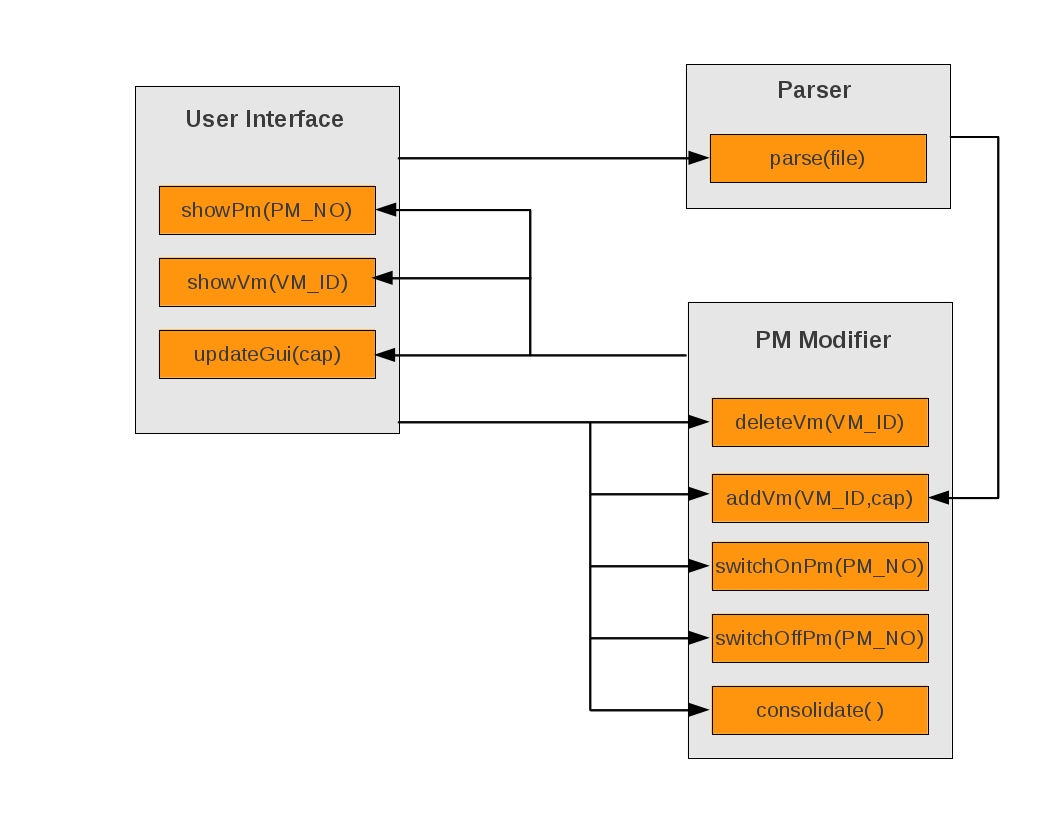
\includegraphics[height=9cm]{images/intrfc.jpg}
%\caption{Interfaces between modules}
%\label{fig:interfaces}
%\end{figure}

\pagebreak
\subsection{Data flow diagram}

%\begin{figure}[h]
%\centering
%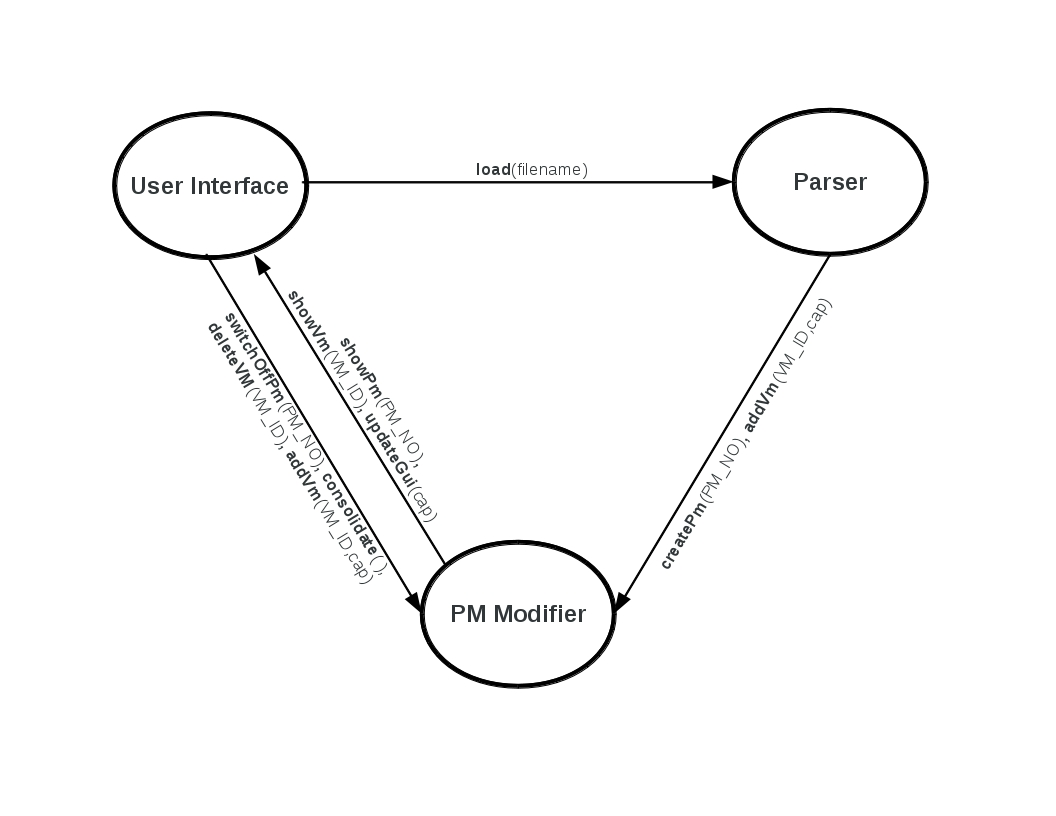
\includegraphics[height=11cm]{images/dfd.jpg}
%\caption{Data flow diagram}
%\label{fig:modules}
%\end{figure}




\subsection{API Specification}
\subsubsection{Modules of the architecture }
\textbf{User Interface Module}
\begin{itemize}
 \item \textbf{Functionality}
 
 The main purpose of this module is to take input from the user and reflect the system state to the user.
 \end{itemize}

\begin{itemize}
\item \textbf{Functionality}

The aim of this module is to parse a text file specified by the user, extract the information about PM's and VM's in it.
It then initializes the PM's which are homogenous and have capacity of 100. Adds VM's to them by the help of PM modifier module.



\textbf{parse(filename)}
  
\begin{tabbing}
\hspace*{3.2cm}\= \kill
 \textit{Purpose} \> :The purpose of this function is to parse the file specified by the \\ \>user and extract information about PM's and VM's.\\
  \textit{Input Parameter} \> : file path specified by the user \\
  \textit{Output Parameter} \> : none \\
  \textit{Return Value} \> : If the file is not in the specified format it would display \\ \>\textbf{wrong file format} message \\
  \textit{Called by} \> : User Interface module \\
  \textit{Calls} \> : createPM and addVM functions of PM modifier\\
  \textit{Data type} \> : \textbf{file} - Class File
\end{tabbing}
\end{itemize}
\textbf{PM modifier}
\begin{itemize}
\item \textbf{Functionality}

The operations of this module includes adding VM's to PM, calculating the residual capacity and consolidation.

\item \textbf{Interface Description}


\textbf{addVm(VM\textunderscore ID, cap)}
  
\begin{tabbing}
\hspace*{3.2cm}\= \kill
 \textit{Purpose} \> : The purpose of this function is to add VM's to the \\ \>PM as specified by the parser.\\
  \textit{Input Parameters} \> : VM ID and VM capacity. \\
  \textit{Output Parameter} \> : none \\
  \textit{Return Value} \> : If there is no enough space to add VM to a PM it outputs \\ \>\textbf{No enough space} message\\
  \textit{Called by} \> : Parser module \\
  \textit{Calls} \> : none.\\
  \textit{Data type} \> : \textbf{VM\textunderscore ID} - Class VMstruct, \textbf{cap} - int
\end{tabbing}

\textbf{deleteVm(VM\textunderscore ID)}
  
\begin{tabbing}
\hspace*{3.2cm}\= \kill
 \textit{Purpose} \> : The purpose of this function is to delete a VM\\ \> specified by the user.\\
  \textit{Input Parameters} \> : PM number in which VM resides and VM ID. \\
  \textit{Output Parameter} \> : none \\
 \textit{Called by} \> : User Interface module \\
  \textit{Calls} \> : none.\\
  \textit{Data type} \> : \textbf{VM\textunderscore ID} - Class VMstruct
\end{tabbing}
\textbf{switchOffPm(PM \textunderscore NO)}
  
\begin{tabbing}
\hspace*{3.2cm}\= \kill
 \textit{Purpose} \> : The purpose of this function is to switch off a PM\\ \> specified by user.\\
  \textit{Input Parameters} \> : PM number. \\
  \textit{Output Parameter} \> : none \\
  \textit{Return Value} \> : Displays \textbf{It is not possible to switchoff this } \\ \>\textbf{PM at this time} if switching off was not successful. \\
  \textit{Called by} \> : User Interface module \\
  \textit{Calls} \> : none.\\
  \textit{Data type} \> : \textbf{PM\textunderscore ID} - Class PMstruct
\end{tabbing}
\textbf{switchOnPm(PM\textunderscore NO)}
\begin{tabbing}
\hspace*{3.2cm}\=\kill
\textit{Purpose}\>: The purpose of this function is to switch on a PM \\ \>specified by user. \\
\textit{Input Parameters}\>: PM number.\\
\textit{Output Parameters}\>: none\\
\textit{Return Value}\>:\\
\textit{Called by}\>: User Interface module\\
\textit{Calls}\>: none.\\
\textit{Data type} \> : \textbf{PM\textunderscore ID} - Class PMstruct
\end{tabbing}
\pagebreak
\textbf{consolidate( )}
  
\begin{tabbing}
\hspace*{3.2cm}\= \kill
 \textit{Purpose} \> : The purpose of this function is to run Bin packing\\ \> algorithm and consolidate all the VM's into minimum number of PM's.\\
  \textit{Input Parameters} \> : none \\
  \textit{Output Parameter} \> : none \\
    \textit{Called by} \> : User Interface module \\
  \textit{Calls} \> : none.\\
\end{tabbing}
\textbf{status( )}
  
\begin{tabbing}
\hspace*{3.2cm}\= \kill
 \textit{Purpose} \> : The purpose of this function is to inform the User Interface\\ \> module the current staus of all the PMs all the VMs in it.\\
  \textit{Input Parameters} \> : none \\
  \textit{Output Parameter} \> : head of the linked list of PMs \\
    \textit{Called by} \> : User Interface module \\
  \textit{Calls} \> : none.\\
  \textit{Data type} \> : \textbf{PM\textunderscore ID} - Class PMstruct
\end{tabbing}
\end{itemize}

\end{document}